% Chapter 2

\chapter{Stochastische Hintergründe}
In diesem Kapitel werden wir erläutern, wie man stochastische Einflüsse auf die KGG darstellen kann. Anschließend werden wir mit der Monte-Carlo Methode bereits ein erstes Verfahren kennen lernen, um den Erwartungswert und die Varianz der zufallsabhängigen Lösung der KGG zu bestimmen.


\section{Grundbegriffe}
Wir geben keine Einführung in die klassische Wahrscheinlichkeitstheorie, werden aber die relevanten Begriffe und Definitionen an dieser Stelle kurz wiederholen. Es sei angemerkt, dass neben den vorgestellten stetigen Verteilungen auch diskrete Verteilungen wie die Poisson-Verteilung existieren und sich durch die selbe Theorie beschreiben lassen. Um die Notation zu vereinfachen, werden wir jedoch ausschließlich stetige Verteilungen betrachten.

\begin{mathdef}[Wahrscheinlichkeitsraum]
Ein Wahrscheinlichkeitsraum $(\Omega,\mathcal{F},P)$ ist ein Tripel bestehend aus 
\begin{itemize}
\item der abzählbaren nichtleeren Ergebnismenge $\Omega$
\item der $\sigma$-Algebra der Ereignisse $\mathcal{F}$ über der Grundmenge $\Omega$
\item dem Wahrscheinlichkeitsmaß $P\colon\mathcal{F}\to [0,1]$
\end{itemize}
\end{mathdef}

\begin{mathdef}[Verteilungsfunktion]
Die Verteilungsfunktion $F_Y$ der Zufallsvariablen $Y\colon\Omega\to\R$ ist definiert durch
\[F_Y(y)\coloneqq P(Y\le y)=P(\left\lbrace \omega\in\Omega |\: Y(\omega)\le y\right\rbrace),\quad y\in\R\]
\end{mathdef}
\begin{mathdef}[Dichte einer Verteilung]
Existiert zu der Verteilungsfunktion $F_Y$ der Zufallsvariablen $Y\colon\R\to\R$ eine Funktion $\rho_Y\colon\R\to\R_{\ge 0}$ mit
\[F_Y(y)=\int_{-\infty}^y\rho_Y(z)dz,\quad y\in\R\]
so nennen wir diese die Dichte von $F_Y$.
\end{mathdef}
\begin{mathdef}[Stochastische Unabhängigkeit]
Ist $(\Omega,\mathcal{F},P)$ ein Wahrscheinlichkeitsraum und $Y_1, Y_2\colon \Omega\to\R$ zwei reelle Zufallsvariablen, so nennt man $Y_1$ und $Y_2$ (stochastisch) unabhängig, genau dann wenn
\[P(Y_1\in B_1,Y_2\in B_2)=P(Y_1\in B_1)P(Y_2\in B_2)\]
für alle $B_1,B_2\in \mathcal{B}(\R)$, der Borelschen $\sigma$-Algebra über $\R$.
\end{mathdef}
\begin{mathbsp}
Ist $\mathcal{N}(\mu, \sigma^2)$ die Normalverteilung mit Parametern $\mu\in\R$ und $\sigma^2>0$ so gilt für ihre Dichtefunktion
\[\rho_Y(y)=\frac{1}{\sqrt{2\pi\sigma^2}}e^{-\frac{(y-\mu)^2}{2\sigma^2}},\quad y\in\R\]
Ist $\mathcal{U}(a,b)$ die Gleichverteilung auf $(a,b)$ so gilt für ihre Dichtefunktion
\[\rho_Y(y)=\begin{cases}\frac{1}{b-a},\quad &y\in (a,b)\\ 0, \quad &\text{sonst} \end{cases}\]
\end{mathbsp}
Folgende Definitionen werden die später hauptsächlich untersuchten Eigenschaften von zufallsabhängigen Größen darstellen.
\begin{mathdef}[Erwartungswert und Varianz]
Ist $Y\colon\R\to\R$ eine reelle Zufallsvariable mit Dichte $\rho_Y$ so ist definieren wir den Erwartungswert von $Y$ als
\[\mu_Y=\E[Y]=\int_{-\infty}^\infty y\rho_Y(y)dy\]
und die Varianz von $Y$ als 
\[\mu_Y^2=\text{var}(Y)=\int_{-\infty}^\infty (y-\mu_Y)^2\rho_Y(y)dy\]
\end{mathdef}
Ohne Beweis präsentieren wir die Inversionsmethode. Diese ist nützlich, um aus Zufallsvariablen einer bestimmten Verteilung Zufallsvariablen einer anderen Verteilung zu gewinnen. In der Numerik ist dies ist essentiell für die Generation von Pseudozufallszahlen von beliebigen Verteilungen, aber auch für die "`stochastische Normierung"' von verschiedenen Zufallsvariablen zu einem gemeinsamen Wahrscheinlichkeitsraum, auf dem dann Erwartungswerte berechnet werden können.
\begin{maththeorem}[Inversionsmethode]
\label{thinversionsmethode}
Ist $Y$ eine reelle Zufallsvariable mit Verteilungsfunktion $F_Y$, so definieren wir deren Quantilfunktion als
\[F_Y^{-1}(p)\coloneqq \inf\lbrace y\in\R |\: F_Y(y)\ge p\rbrace,\quad p\in\R\]
Dann gilt
\begin{itemize}
\item $z\le F_Y(y)\iff F_Y^{-1}(z)\le y$\\
\item Falls $Z$ gleichverteilt in $(0,1)$ ist, dann hat $F_Y^{-1}(Z)$ die Verteilungsfunktion $F_Y$. 
\end{itemize}
\end{maththeorem}
Der auch Gesetz der großen Zahlen genannte Zentrale Grenzwertsatz sei ebenfalls genannt, da er die Grundlage für das erste Verfahren zur Berechnung von Erwartungswert und Varianz darstellt.
\begin{maththeorem}[Zentraler Grenzwertsatz]
\label{thzentralgrenzwert}
Seien $Y_1,Y_2,\dots,Y_n$ unabhängige und identisch verteilte Zufallsvariablen mit $\E[Y]_i=\mu$ und $\text{var}(Y_i)=\sigma^2<\infty$ Der Mittelwert sei definiert als
\[\overline{Y}\coloneqq \frac{1}{n}\sum_{i=1}^nY_i\]
und skaliert durch
\[Z_n=\sqrt{n}\left(\frac{\overline{Y}-\mu}{\sigma}\right)\]
Dann konvergiert für $n\to\infty$ die Verteilungsfunktion von $Z_n$ zu einer $\mathcal{N}(0,1)$ verteilten Verteilungsfunktion.
\end{maththeorem}
\begin{mathdef}[Zufallsvektoren]
Wir nennen $Y=(Y_1,\dots,Y_n)$ einen $n$-dimensionalen Zufallsvektor (häufig auch einfach $n$-dimensionale Zufallsvariable), wenn die Komponenten $Y_1,\dots,Y_n\colon\Omega\to\R$ eindimensionale Zufallsvariablen sind. Besitzt jede Komponente $Y_i$ eine Dichte $\rho_{Y_i}$, so ist die gemeinsame Dichte
\[\rho_Y=\prod_{i=1}^n \rho_{Y_i}\]
und die Verteilungsfunktion lässt sich darstellen als
\[F_Y(y_1,\dots,y_n)=\int_{-\infty}^{y_1}\dots\int_{-\infty}^{y_n}\rho_Y(z_1,\dots,z_n)dy_1\dots dy_n\]
\end{mathdef}
Weitere wichtige Begriffe, die aber in dieser Arbeit nicht in den Vordergrund rücken werden, seien stichwortartig genannt:
\begin{itemize}
\item Konvergenz $P$ fast sicher, Konvergenz in Wahrscheinlichkeit, Konvergenz in Verteilung\\
\item Bedingte Wahrscheinlichkeit, bedingte Erwartung
\item Unkorreliertheit vs. Unabhängigkeit
\item Momente höherer Ordnung, Moment-generierende Funktion
\end{itemize}

\section{Endliche Parametrisierung}
\label{secfiniteparam}
Dieser Abschnitt beschäftigt sich mit der Frage, wie man, ausgehend von einem potentiell unendlich dimensionalen Wahrscheinlichkeitsraum, eine endliche Charakterisierung desselben durch einen $n$-dimensionalen Zufallsvektor mit unabhängigen Komponenten erhalten kann. Die Bedingung der Unabhängigkeit ist dabei theoretisch zwar wenig einschränkend, aber eine sehr wichtige Grundlage für viele praktische numerische Verfahren.\\
Diese Frage tritt beispielsweise auf, wenn die Zufallsabhängigkeit im Modell nicht explizit über die Parameter einfließt, sondern ein zeitabhängiger stochastischer Prozess ist. Möglich wäre auch, dass die Zufallsabhängigkeit in endlich oder abzählbar vielen Modellparametern steckt, die einzelnen Parameter jedoch nicht stochastisch unabhängig sind.\\
Wir werden später stets davon ausgehen, dass bereits eine endliche Parametrisierung durch unabhängige Zufallsvariablen mit bekannter Verteilung vorliegt. Der Vollständigkeit aber seien hier kurz Methoden genannt, um das Parametrisierungsproblem zu lösen. Man beachte jedoch, dass einige der Methoden numerisch nicht umsetzbar oder ad-hoc Lösungen sind, die spezielle Annahmen benötigen. Dieser Abschnitt wurde aus \autocite[Kapitel 4.1+4.2]{dongbinxiu2010} übernommen, wo auch Visualisierungen und kleine Beispiele zu finden sind.

\subsection{Unabhängigkeit von endlich vielen Parametern}
Wenn die Zufallsabhängigkeit des Modells bereits durch endlich viele Modellparameter vorliegt, ist die Parameterisierung bereits gegeben. Wichtig ist dann, die unabhängigen Parameter zu identifizieren bzw. die Abhängigkeit zu konkretisieren.\\
Für normalverteilte Parameter ist dies auch auf einfache Weise möglich:
\begin{maththeorem}
\label{thgaussunabhg}
Sei $Y=(Y_1,\dots,Y_n)$ ein $\mathcal{N}(0,C)$ verteilter Zufallsvektor mit Kovarianzmatrix $C\in\R^{n\times n}$. Sei $Z\sim\mathcal{N}(0,I_n)$, wobei $I_n$ die n-dimensionale Einheitsmatrix ist, ein unkorrelierter Zufallsvektor. Für die Gaussverteilung ist Unkorreliertheit äquivalent zu Unabhängigkeit und die Komponenten von $Z$ sind somit unabhängig. Da $C$ reell und symmetrisch ist, existiert die Choleskyzerlegung $C=AA^T$ und es gilt
\[Y=AZ\sim\mathcal{N}(0,AA^T)=\mathcal{N}(0,C)\]
besitzt die gegebene Verteilung. Wir können folglich $Y$ durch stochastisch unabhängige Parameter $Z_1,\dots,Z_n$ darstellen.
\end{maththeorem}
Sind die Parameter nicht normalverteilt, so wird das Problem deutlich schwieriger und bis jetzt gibt es keine zufriedenstellende numerische Transformation, die entsprechendes zu Satz \ref{thgaussunabhg} leistet. Eine theoretische Möglichkeit bietet sich jedoch über die Rosenblatt Transformation, welche auf den in der Praxis selten bekannten bedingten Wahrscheinlichkeiten basiert.

\subsection{Parametrisierung von Zufallsprozessen}
Häufig sind die Zufallsabhängigkeiten des Modells nur durch Beobachtungen oder Messungen von Zufallsvariablen möglich. Wir schreiben diese als stochastischen Prozess $(Y_t,t\in T)$, wobei $T$ der Indexraum ist und $Y_t$ die beobachteten Zufallsvariablen. Wir suchen dann eine Transformation $R$, welche die Darstellung $Y_t=R(Z)$ mit Zufallsvektor $Z=(Z_1,\dots,Z_n)$ und unabhängigen Komponenten $Z_i$ erlaubt. Da $T$ potentiell ein unendlich dimensionaler Raum ist, kann diese Transformation nicht exakt sein und wir suchen nun eine in einem gewissen Sinne bestmögliche Approximation.\\
Die am häufigsten verwendete Technik ist dabei die Karhunen-Loeve Reihendarstellung.
\begin{mathdef}[Karhunen-Loeve Darstellung]
Sei $\mu_Y(t)$ der Erwartungswert des Prozesses $Y_t$ am Punkt $t$ und sei $C(t,s)=\text{cov}(Y_t,Y_s)$ die Kovarianzfunktion. Dann ist die Karhunen-Loeve Darstellung definiert als
\[Y_t(\omega)=\mu_Y(t)+\sum_{i=1}^\infty \sqrt{\lambda_i}\Psi_i(t)Z_i(\omega)\] wobei $\Psi_i$ die orthogonalen Eigenfunktionen und $\lambda_i$ die zugehörigen Eigenwerte des Eigenwertproblems
\[\int_T C(t,s)\Psi_i(s)ds=\lambda_i\Psi_i(t),\quad t\in T\]
sind. Die paarweise unkorrelierten Zufallsvariablen $Z_i(\omega)$ erfüllen
\[\E[Z_i]=0,\quad \E[Z_iZ_j]=\delta_{ij}\]
und sind definiert durch
\[Z_i(\omega)=\frac{1}{\sqrt{\lambda_i}}\int_T (Y_t(\omega)-\mu_Y(t))\Psi_i(t)dt\]
Um eine endliche Approximation zu erhalten wird die Reihe bei einem gewissen Index $n\in\N$ abgebrochen.
\end{mathdef}
Wiederrum erhält man daraus für normalverteilte Prozesse eine endliche Menge von unabhängigen Zufallsvariablen. Für nicht-normalverteilte Prozesse wird häufig dennoch die Karhunen-Loeve Darstellung verwendet und zusätzlich angenommen, dass die $Z_i$ unabhängig sind. Diese Vorgehensweise ist noch nicht zufrieden stellend und ein offenes Forschungsproblem.

\section{Formulierung der stochastischen KGG}
In Analogie zur Klein-Gordon-Gleichung (\ref{kgg}) definieren wir für einen Wahrscheinlichkeitsraum $(\Omega,\mathcal{F},P)$ und $Y\colon\Omega\to\R^N$ die stochastische Klein-Gordon-Gleichung (sKGG) für $y=Y(\omega)$ durch
\begin{align}
\label{skgg}
\dtt{u}(t,x,y)&=\alpha(y) \Laplace_x u(t,x,y) - \beta(x,\omega)u(t,x,y), \: t>0, \, x\in \Torus^d\\
u(0,x,y)&=u_0(x,y), \: x\in \Torus^d\\
\dt{u}(0,x,y)&=v_0(x,y), \: x\in \Torus^d
\end{align}
Die Lösung \[u(t,x,y)\colon [0,T]\times\Torus^d\times \R^N\to\R\] ist also eine zufallsabhängige Größe.\\
Dabei ist die grundlegende Annahme, dass (\ref{skgg}) $P$-fast-sicher wohl gestellt ist, d.h. die Menge an Punkten $\omega$ für welche die partielle Differentialgleichung mit fixem $y=Y(\omega)$ keine eindeutige Lösung besitzt ist eine Nullmenge bezüglich des Wahrscheinlichkeitmaßes $P$.\\
Ab sofort werden wir --wie in Kapitel \ref{secfiniteparam} diskutiert-- stets annehmen, dass die Komponenten $Y_i$ von $Y$ stochastisch unabhängige Zufallsvariablen mit bekannter Verteilung sind.
\begin{mathbsp}
Sei $Y=(Y_1)$ eine eindimensionale und in $(2,3)$ gleichverteilte Zufallsvariable. Dann gilt für $t>0$, $d\in\N$, $x=(x_1,\dots$, $x_d)\in\Torus^d$, $\hat{x}\coloneqq \sum_{i=1}^d x_i$ und $y=Y(\omega)$
\begin{align*}
u(t,x,y)&=2\cos(ty)\sin(\hat{x})\\
u_0(x,y)&=2\sin(\hat{x})\\
v_0(x,y)&\equiv 0
\end{align*}
löst die stochastische KGG (\ref{skgg}) für $\alpha(y)=\frac{y}{d}$ und $\beta(x,y)=y^2-y$\\
Für den Erwartungswert und Varianz von $u$ gelten
\begin{align*}
\E[u(t,x,Y)]&=\int_2^3u(t,x,y)dy=\frac{2}{t}\sin(\hat{x})(\sin(3t) - \sin(2t))\\
\text{var}(u(t,x,Y))&=\frac{1}{t}\sin^2(\hat{x})\left(2t + \sin(6t) - \sin(4t)\right)- \left(\frac{2}{t}\sin(\hat{x})(\sin(3t) - \sin(2t))\right)^2
\end{align*}
Um einen potentiellen Denkfehler zu vermeiden, weisen wir an dieser Stelle explizit darauf hin, dass 
\[\E[u(t,x,Y)]=\frac{2}{t}\sin(\hat{x})(\sin(3t) - \sin(2t))\neq 2\sin(\hat{x})\cos(\frac{5}{2}t)=u(t,x,\E[Y])\]
Dies erkennt man beispielsweise am Zeitpunkt $t=\frac{\pi}{2}$, wo gilt
\[\E[u(t,x,Y)]=-\sin(\hat{x})\pi \neq -\sin(\hat{x})\sqrt{2}=u(t,x,\E[Y])\]
Der Erwartungswert ist linear, die Abhängigkeiten von $y$ sind es aber nicht. Diese erste fehlgeschlagene Idee den Erwartungswert durch das Lösen eines deterministischen Systems zu erhalten, ist jedoch nicht vollends vergebens. Wir werden am Beispiel der Monte-Carlo-Methode sehen, dass wir dazu allerdings weit mehr als ein System lösen müssen.
\end{mathbsp}
Wir geben ein weiteres Referenzbeispiel an, wo nun auch die Ortsabhängigkeit von $\beta$ benutzt wird und auch ein Anfangswert abhängig von der Zufallsvariablen ist.
\begin{mathbsp}
Sei $Y=(Y_1)$ eine eindimensionale und in $(10,50)$ gleichverteilte Zufallsvariable. Dann gilt für $t>0$, $d=1$, $x\in\Torus$ und $y=Y(\omega)$
\begin{align*}
u(t,x,y)&=\frac{\cos(t)}{\sin(x) + y}\\
u_0(x,y)&=\frac{1}{\sin(x) + y}\\
v_0(x,y)&\equiv 0
\end{align*}
löst die stochastische KGG (\ref{skgg}) für \[\alpha(y)=y-2\text{  und  }\beta(x,y)=1 + (y-2)\left(\frac{\sin(x)}{\sin(x) + y}+ \frac{2\cos^2(x)}{(\sin(x) + y)^2}\right)\]
Für den Erwartungswert von $u$ gilt
\[\E[u(t,x,Y)]=\frac{\cos(t)}{40}(\log(\sin(x) + 50)- \log(\sin(x) + 10))\]
\end{mathbsp}
\section{Die Monte-Carlo-Methode} % offizieller Name; auch: Monte-Carlo-Simulation
Die Monte-Carlo-Methode (auch: Monte-Carlo-Simulation) ist ein in vielen Disziplinen bekanntes Verfahren, welches auf wiederholtem Durchführen von "`Zufallsexperimenten"' in sehr großer Zahl basiert. So können analytisch nicht --oder nur sehr aufwändig-- lösbare Probleme auf Basis des Gesetz der großen Zahlen approximiert werden.\\
Die Grundstruktur des Algorithmus, angewandt auf die stochastische KGG zur Berechnung des Erwartungswertes und der Varianz, ist beschrieben durch Algorithmus \ref{algmc}.
\begin{algorithm}[ht]
    \caption{Monte-Carlo}
    \label{algmc}
    \begin{algorithmic}[1] % The number tells where the line numbering should start
        \Function{MonteCarloKGG}{$u_0,v_0,\alpha,\beta,Y,max\_runs$} 
            \State $r\gets 0$
            \While{$r<max\_runs$} \Comment{Stoppen nach fixer Anzahl Durchläufen}
                \State $y \gets Y(\omega)$ \Comment{Generiere zufälliges $y$ nach geg. Verteilung}
                \State Berechne deterministische Parameter $u_0(x,y)$, $v_0(x,y)$, $\alpha(y)$ und $\beta(x,y)$
                \State Löse KGG (\ref{skgg}) mit deterministischen Parametern
                \State Speichere Lösung der KGG
                \State $r\gets r+1$
            \EndWhile
            \State $e\gets$ Mittelwert der gespeicherten Lösungen
            \State $v\gets$ Schätzung der Varianz der gespeicherten Lösungen
            \State \textbf{return} $e, v$\Comment{Geschätzter Erwartungswert und Varianz}
        \EndFunction
    \end{algorithmic}
\end{algorithm}
Doch die Pseudocode Beschreibung von der Funktion \emph{MonteCarloKGG} wirft einige neue Fragen auf:
\begin{enumerate}
\item Wie generieren wir die Zufallszahlen numerisch? \label{mcgeneraterandom}
\item Wie groß muss \emph{\texttt{max\_runs}} sein, d.h. wie schnell konvergiert die Methode?
\item Ist der determinische Löser schnell genug für viele Durchläufe? Wie können wir den Algorithmus beschleunigen?\label{mcalgspeed}
\item Wie speichern wir die vielen Zwischenergebnisse? \label{mcsaveresults}
\item Wie berechnen wir den Mittelwert und wie schätzen wir die Varianz? \label{mcestimations}
\end{enumerate}
Im Folgenden werden wir die obigen Fragen ausführlich diskutieren und verschiedene Möglichkeiten aufzeigen, sie zu beantworten.
\subsection{Generierung von Pseudozufallszahlen}
Eine Antwort auf Frage \ref{mcgeneraterandom} zur Generierung von $y$ ist durch das Schlagwort "`Pseudozufallszahlen"' direkt gegeben. Hierzu bietet jede wissenschaftliche Programmiersprache die Möglichkeit, Zahlen zu generieren, die zwar deterministisch erzeugt sind, jedoch viele Eigenschaften von Zufallszahlen erfüllen. Dabei wird häufig eine große Menge von bekannten Verteilungen unterstützt. Ist dies nicht der Fall und man hat beispielsweise nur gleichverteilte Zahlen zur Verfügung, so kann man dennoch mithilfe der Inversionsmethode (siehe Satz \ref{thinversionsmethode}) Pseudozufallszahlen mit jeder beliebigen Verteilungsfunktion erzeugen.\\
Dies ist jedoch weder die einzige noch die beste Möglichkeit für die Generierung.
\subsubsection*{Quasi-Monte-Carlo-Methode}
Eine weitere Möglichkeit für die Generierung von Sequenzen, die sich in vielen Aspekten wie Zufallszahlen verhalten, ist durch sogenannte \emph{low discrepancy} Sequenzen wie der Halton-Sequenz gegeben. Diese Sequenz wurde von Halton in \autocite{halton60} vorgestellt und bieten eine Alternative zu $N$-dimensionalen in $(0,1)^N$ gleichverteilten Pseudozufallszahlen auf Basis der Van-der-Corput-Sequenz.\\
\begin{mathdef}[Van-der-Corput-Sequenz]
Die Van-der-Corput-Sequenz zu einer Basis $b\in\N$ ist definiert durch die Folge $(c_b(n))_{n\in\N}$ wobei
\begin{equation*}
n=\sum_{k=0}^{L-1}d_k(n)b^k
\end{equation*}
die Darstellung von $n$ zur Basis $b$ ist und
\begin{equation*}
c_b(n)=\sum_{k=0}^{L-1}d_k(n)b^{-k-1}
\end{equation*}
\end{mathdef}
\begin{mathdef}[Halton-Sequenz]
Die Halton-Sequenz zu einer Dimension $N\in\N$ ist definiert als die Folge $(c_{p_1}(n),\dots,c_{p_N}(n))_{n\in\N}$, wobei $p_1,\dots,p_N\in\N$ die ersten $N$ Primzahlen sind und $c_p(n)$ die $n$-te Van-der-Corput Zahl.
\end{mathdef}
\begin{mathbsp}
Beispielsweise ist für $p=3$ die $n=5$-te Van-der-Corput Zahl gegeben durch 
\begin{align*}
5&=1\cdot 3^1+2\cdot 3^0=12_3\\
c_3(5)&=1\cdot 3^{-2}+2\cdot 3^{-1}=0.21_3=\frac{7}{9}
\end{align*}
Die Halton-Sequenz für $N=2$ Dimensionen beginnt mit den Zahlen
\begin{equation*}
(c_2(n),c_3(n))_{n\in\N}=\left(\left(\frac{1}{2},\frac{1}{3}\right),\left(\frac{1}{4},\frac{2}{3}\right),\left(\frac{3}{4},\frac{1}{9}\right),\left(\frac{1}{8},\frac{4}{9}\right),\left(\frac{5}{8},\frac{7}{9}\right),\left(\frac{3}{8},\frac{2}{9}\right),\dots\right)
\end{equation*}
\end{mathbsp}
In höheren Dimensionen (ab ungefähr $N=6$) beobachtet man allerdings stärkere lineare Korrelation zwischen den Komponenten, siehe beispielsweise Sequenzen für $p=17$ und $p=19$. Die Komponenten sind also abhängig und somit kein guter Ersatz für Pseudozufallszahlen. Genauere Untersuchungen werden in \autocite{Morokoff1995218} erläutert, wo auch vorgeschlagen wird für höhere Dimensionen die Sobol-Sequenz zu verwenden.\\
Wie man an Abbildung \ref{fig:halton_numbers} erkennt, deckt die Halton-Sequenz die Fläche deutlich gleichmäßiger ab als eine Generierung von der selben Anzahl an Pseudozufallszahlen. Dies ist eine Motivation dafür, bessere Konvergenzeigenschaften zu erwarten.
\begin{figure}
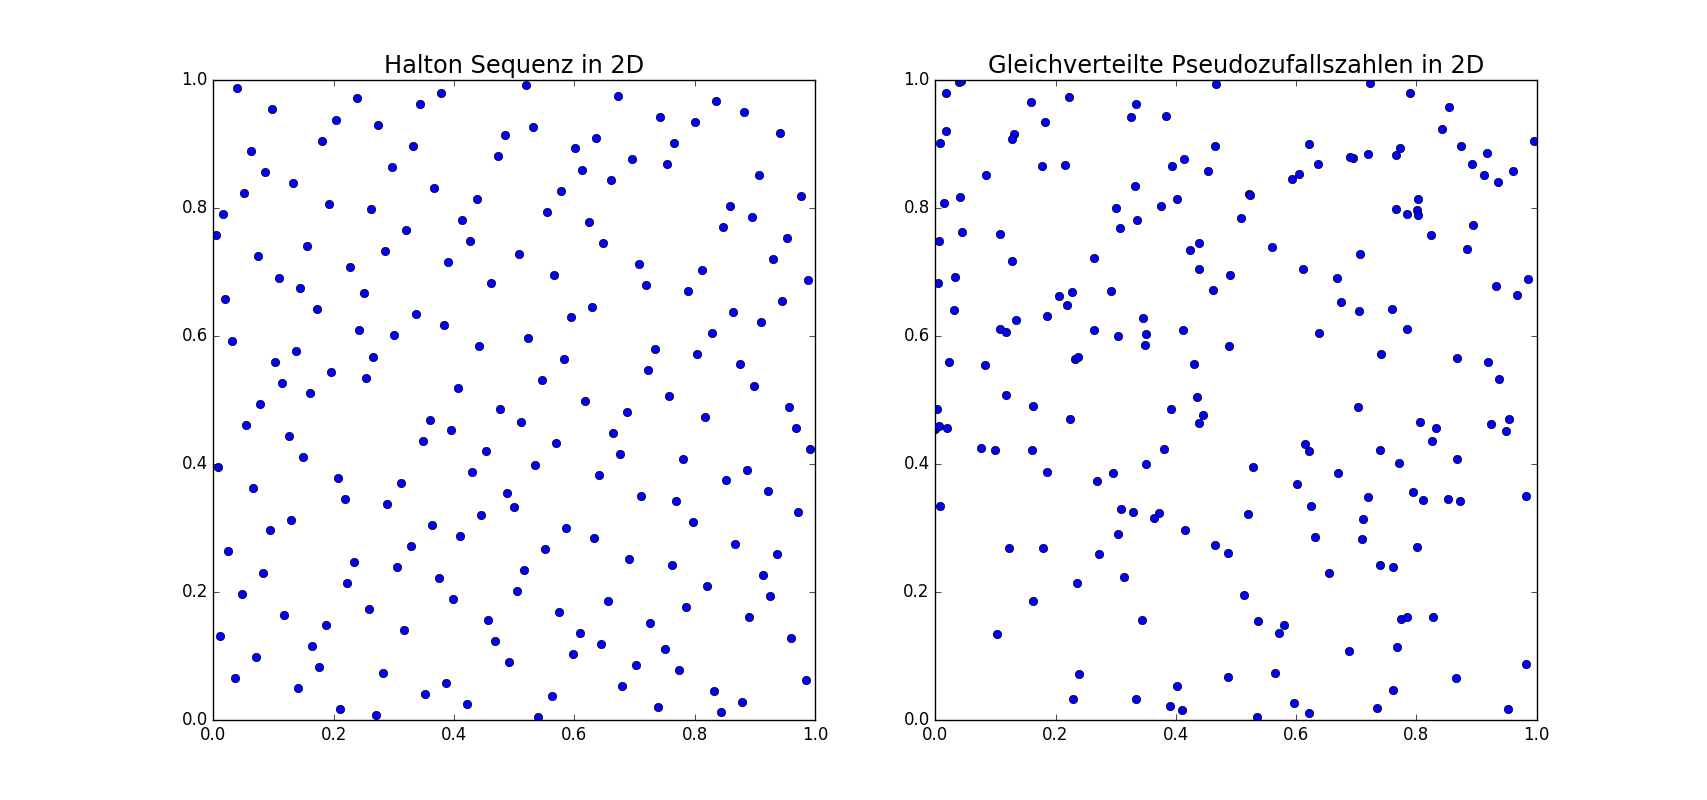
\includegraphics[width=\textwidth]{Figures/halton_numbers.png}
\caption{Darstellung der ersten 200 Halton Zahlen im zweidimensionalen und im Vergleich 200 gleichverteilte Pseudozufallszahlen. Die Halton Sequenz deckt die Fläche dabei viel gleichmäßiger ab.}
\label{fig:halton_numbers}
\end{figure}
Benötigt man wiederum Zufallszahlen mit einer anderen Verteilungsfunktion, so sind diese durch Anwendung der Inversionsmethode \ref{thinversionsmethode} erzeugbar.

\subsection{Approximation von Erwartungswert und Varianz}
Bevor wir den Kern der Schleife betrachten, wollen wir uns zuerst mit den eng miteinander zusammenhängenden Fragen \ref{mcsaveresults} und \ref{mcestimations} beschäftigen. Diese Fragen über die Verwendung der einzelnen Zwischenergebnisse zur Approximation des Erwartungswertes und der Varianz können wiederum vielseitig beantwortet werden.
\subsubsection*{Verarbeitung am Ende}
Gegeben sei ein Zeitpunkt $T>0$ und die stochastische KGG (\ref{skgg}) zu einer Zufallsvariablen $Y$ und gesucht seien $\E[u(T,x,Y)]$ und $\text{var}(u(T,x,Y))$. Sind für $i=1,\dots,R$ die deterministischen Lösungen $u_i(T,x,y_i)$ gespeichert, so verwenden wir als Approximationen
\begin{align*}
\E[u(T,x,Y)]&\approx \frac{1}{R}\sum_{i=1}^R u_i(T,x,y_i)\eqqcolon m_R\\
\text{var}(u(T,x,Y)) &\approx \frac{1}{R-1}\sum_{i=1}^R(u_i(T,x,y_i)-m_R)^2
\end{align*}
Wieso diese Approximationen sinnvoll sind, zeigt sich teilweise aus dem zentralen Grenzwertsatz \ref{thzentralgrenzwert}. Es folgt für unabhängige Stichproben $y_i$ die Aussage \[\sqrt{R}(m_R-\E[u(T,x,Y)])\xrightarrow{R\to\infty}\mathcal{N}(0,\text{var}(u(T,x,Y)))\]
und schlussendlich 
\[m_R=\E[u(T,x,Y)] + \mathcal{O}\left(\frac{1}{\sqrt{R}}\right)\]
In welchem Konvergenz Sinne die letzte Aussage zu verstehen ist und welche Faktoren dabei in den letzten Term einfließen, sei an dieser Stelle nicht weiter ausgeführt. Wir werden diese Konvergenzordnung in Beispielen jedoch empirisch bestätigen.\\[0.2cm]
Die für die Approximation der Varianz verwendete Darstellung nennt man auch \emph{korrigierte Stichprobenvarianz}. Sie ist ein erwartungstreuer Schätzer der Varianz einer Stichprobe und ein Werkzeug aus der Statistik, welches wir hier nicht weiter erläutern werden.
\subsubsection*{Fortlaufende Berechnung}
Die Verarbeitung am Ende besitzt zwei große Nachteile:
\begin{itemize}
\item Sämtliche Zwischenergebnisse müssen gespeichert werden. Für die Mittelwertbildung alleine wäre dies zwar nicht nötig, jedoch für die Approximation der Varianz. An einer Beispielsrechnung soll der benötigte Arbeitsspeicher kurz verdeutlicht werden: Wird der Raum in 256 Punkten diskretisiert und benötigt jeder Punkt 8 Byte Speicher und führt man (durchaus realistisch) $R=100000$ Simulationen durch, so ergibt sich bereits ein Speicherbedarf von $\frac{256*100000*8\text{B}}{1024^2}\approx 200\text{MB}$. Dies ist also bereits für eine räumliche Dimension ein nicht unerheblicher Aufwand.
\item Die Methode zur Approximation der Varianz ist nicht stabil und stark anfällig für numerische Rechenfehler, insbesondere Überläufe (vgl. \autocite{cook08}). Aus diesem Grunde schlug Welford in \autocite{welford62} eine alternative Berechnungsmethode vor, welche wir im folgenden erklären werden.
\end{itemize}
\begin{maththeorem}
\label{thiterativemk}
Für $x_1,\dots,x_k\in\R$ und $m_k=\frac{1}{k}\sum_{j=1}^kx_j$ gilt für $k\in\N$ die iterative Darstellung
\[m_k=m_{k-1}+\frac{x_k-m_{k-1}}{k},\quad \text{mit }\: m_0=0\]
\end{maththeorem}
\begin{proof}
Wir zeigen mithilfe vollständiger Induktion die äquivalente Aussage, dass die Rekursion mit der Darstellung $m_k=\frac{1}{k}\sum_{j=1}^kx_j$ übereinstimmt.\\
I.A. ($k=1$): \[m_1=0+\frac{x_1-0}{1}=x_1=\sum_{j=1}^1x_j\quad\surd\]
I.S. ($k\leadsto k+1$):
\begin{align*}
m_{k+1}&\stackrel{Def}{=}m_k+\frac{x_{k+1}-m_k}{k+1}\\
&\stackrel{IV}{=}\frac{1}{k}\sum_{j=1}^kx_j+\frac{x_{k+1}}{k+1}-\frac{1}{k(k+1)}\sum_{j=1}^kx_j
\end{align*}
Multiplizieren wir nun mit $k(k+1)$ so erhalten wir
\begin{align*}
k(k+1)m_{k+1}&=(k+1)\sum_{j=1}^kx_j+kx_{k+1}-\sum_{j=1}^kx_j\\
&=k\sum_{j=1}^{k+1}x_j\\
\implies m_{k+1}&=\frac{1}{k+1}\sum_{j=1}^{k+1}x_j
\end{align*}
\end{proof}
Wir haben nun also eine iterative Methode zur Berechnung des Mittelwertes gewonnen, die nur den vorherigen Mittelwert, die neue Stichprobe und die Anzahl an Stichproben benötigt. Diese Methode ist robust gegen Überläufe und numerisch stabil. Viel wichtiger ist jedoch die iterative Berechnung des Varianzschätzers, welche auf ähnlichen Ideen basiert. Die Äquivalenz zur ursprünglichen Methode ist dabei allerdings schwieriger zu erkennen.
\begin{maththeorem}
Für $x_1,\dots,x_k\in\R$, $m_k$ wie in Satz \ref{thiterativemk} und $s_k=\sum_{j=1}^k(x_j-m_k)^2$ gilt für $k\in\N$ die iterative Darstellung
\[s_k=s_{k-1}+(x_k-m_k)(x_k-m_{k-1}),\quad\text{mit }s_0=0\]
\end{maththeorem}
\begin{proof}
Es gilt für $j<k$ wegen $m_k=\frac{k-1}{k}m_{k-1}+\frac{1}{k}x_k$
\begin{align}
x_j-m_k&=x_j-m_{k-1}+\frac{1}{k}m_{k-1}-\frac{1}{k}x_k \nonumber\\
\label{eqn:mcvar1}
&=x_j-m_{k-1}-\frac{1}{k}(x_k-m_{k-1})\tag{*}\\
\label{eqn:mcvar2}
x_k-m_k&=\frac{k-1}{k}(x_k-m_{k-1})\tag{**}
\end{align}
Dann gilt für $k\in\N$
\begin{align*}
s_k&=\sum_{j=1}^k(x_j-m_k)^2\stackrel{(\ref{eqn:mcvar2})}{=}\sum_{j=1}^{k-1}(x_j-m_k)^2+\frac{(k-1)^2}{k^2}(x_k-m_{k-1})^2\\
&\stackrel{(\ref{eqn:mcvar1})}{=}\sum_{j=1}^{k-1}(x_j-m_{k-1})^2-\frac{2}{k}(x_k-m_{k-1})\sum_{j=1}^{k-1}(x_j-m_{k-1})+\frac{k-1}{k^2}(x_k-m_{k-1})^2\\
&\quad +\frac{(k-1)^2}{k^2}(x_k-m_{k-1})^2\\
&=s_{k-1}-\frac{2}{k}(x_k-m_{k-1})\underbrace{\left((k-1)m_{k-1}-(k-1)m_{k-1}\right)}_{=0}+\underbrace{\frac{(k-1)^2+k-1}{k^2}}_{=\frac{k-1}{k}}(x_k-m_{k-1})^2\\
&=s_{k-1}+\frac{k-1}{k}(x_k-m_{k-1})\underbrace{(x_k-m_{k-1})}_{\stackrel{(\ref{eqn:mcvar2})}{=}\frac{k}{k-1}(x_k-m_k)}=s_{k-1}+(x_k-m_{k-1})(x_k-m_k)
\end{align*}
\end{proof}
Teilen wir nun $s_k$ noch durch $k-1$, so erhalten wir wieder die korrigierte Stichprobenvarianz. Wir benötigen dafür nur den vorherigen Wert $s_{k-1}$, die beiden letzten Mittelwerte, die neuste Stichprobe $x_k$ und die Stichprobenanzahl.
\subsection{Numerische Ergebnisse}
Man bemerkt schon an der Pseudocode Darstellung der Monte-Carlo-Methode, dass das Bottleneck des Algorithmus in der Berechnung der Lösung der deterministischen KGG liegt. Der Zeitaufwand für alle anderen Operationen ist in Relation dazu vernachlässigbar klein. Ein großer Vorteil des Algorithmus ist seine \emph{embarrassingly parallel} Eigenschaft: Es ist quasi kein Aufwand nötig die Schleife zu parallelisieren und somit skaliert er perfekt mit der Anzahl an zur Verfügung stehenden Prozessoren. Dies ist eine erste Antwort auf Frage \ref{mcalgspeed}, jedoch sollte klar sein, dass das Lösen des deterministischen Systems dennoch so effizient wie möglich passieren muss. Ein Löser, der nur 0.1 Sekunden für ein einziges System benötigt und $R=100000$ Durchgänge erledigt, läuft bereits etwa 3 Stunden ohne Parallelisierung.\\

\todo[inline]{Bilder: Konvergenzordnung von MC anhand von bsp1 und 2; Zeige bessere Ordnung und Fehlerverhalten von qMC; Zeige Konvergenzordnung von Varianz; Zeige was R=100000 so bedeutet im Vergleich zu R=317=sqrt(100000); Erwähne Vorteil dass Konvergenz unabhäng von Dim. von y (zeige entsprechendes BSP)}

